\section{Results}
\label{sec:results}

This section presents an evaluation of our JPEG-like compression system across multiple parameter sweeps and test scenarios. The goal is to assess compression performance with respect to visual quality, file size, semantic preservation, and runtime efficiency.

\subsection{Overview of Evaluation Goals}
Our evaluation focuses on the following:
\begin{itemize}
    \item \textbf{Compression Quality}: Comparison of output image quality under various compression settings
    \item \textbf{Compression Ratio}: Size reduction achieved with each configuration
    \item \textbf{Semantic Preservation}: Classification consistency of compressed images using pre-trained models
    \item \textbf{Runtime Performance}: Timing analysis for compression and decompression operations
\end{itemize}

\subsection{Test Methodology}
Experiments are conducted using YAML configurations across:
\begin{itemize}
    \item \texttt{compression\_configurations/\allowbreak quantization\_sweep/}
    \item \texttt{compression\_configurations/\allowbreak downsample\_sweep/}
    \item \texttt{compression\_configurations/\allowbreak block\_size\_sweep/}
    \item \texttt{compression\_configurations/\allowbreak quantization\_sweep\_chroma/}
    \item \texttt{compression\_configurations/\allowbreak quantization\_sweep\_luma/}
    \item \texttt{compression\_configurations/\allowbreak quantization\_sweep\_small\_blocks/}
\end{itemize}

Each configuration is tested on a standardized dataset of images (\texttt{assets/test\_images/}) with various formats and content types. Results are logged in corresponding metrics files (.metrics.json) and visual artifacts are stored in \texttt{results/}.

These additional sweeps were introduced after the initial draft to better isolate compression artifacts and parameter sensitivity across chroma and luma components.

To assist with analysis and visualization, we created a dedicated Jupyter notebook (\texttt{notebooks/plot\_results.ipynb}) to plot trends in PSNR, SSIM, compression ratios, and runtime performance across different sweep parameters.

\subsection{Parameter Sweeps}

To test the sensitivity of our various metrics across a variety of compression parameters, the following parameter sweeps are performed:

\begin{table}[h!]
    \centering
    \caption{Gaussian Quantization Weights Quantization Parameters Tested}
    \begin{tabularx}{0.5\textwidth}{X c c c}
        \toprule
        \ & \textbf{Luma} & \textbf{Chroma} \\
        \ & \textbf{Quantization} & \textbf{Quantization} \\
        \ & \textbf{Max, $\sigma$} & \textbf{Max, $\sigma$} \\
        \midrule
        No Quantization & 1 , 1 & 1, 1 \\
        High Quality & 10,3 & 20, 3 \\
        Quality & 30, 5 & 40, 5 \\
        Moderate Quality & 60, 6 & 75, 6 \\
        Low Quality & 100, 8 & 125, 8 \\
        Very Low Quality & 150, 10 & 200, 10 \\
        \bottomrule
    \end{tabularx}
    \label{tab:Quantization-Parameters-Table}
\end{table}

\begin{table}[h!]
    \centering
    \caption{LN-Norm Quantization Parameters Tested}
    \begin{tabularx}{0.5\textwidth}{X c c c}
        \toprule
        \ & \textbf{Luma} & \textbf{Chroma} \\
        \ & \textbf{Quantization} & \textbf{Quantization} \\
        \ & \textbf{Max, Min} & \textbf{Max, Min} \\
        \midrule
        No Quantization & 1 , 1 & 1, 1 \\
        L1.5 High Quality & 10, 5 & 20, 10 \\
        L1.5 Quality & 40, 20 & 50, 30 \\
        L1.5 Med Quality & 50, 20 & 60, 30 \\
        L1.5 Low Quality & 100, 30 & 125, 40 \\
        L1.5 Very Low Quality & 200, 80 & 150, 60 \\
        L2 High Quality & 10, 5 & 20, 10 \\
        L2 Quality & 40, 20 & 50, 30 \\
        L2 Med Quality & 50, 20 & 60, 30 \\
        L2 Low Quality & 100, 30 & 125, 40 \\
        L2 Very Low Quality & 200, 80 & 150, 60 \\
        L3 High Quality & 10, 5 & 20, 10 \\
        L3 Quality & 40, 20 & 50, 30 \\
        L3 Med Quality & 50, 20 & 60, 30 \\
        L3 Low Quality & 100, 30 & 125, 40 \\
        L3 Very Low Quality & 200, 80 & 150, 60 \\
        \bottomrule
    \end{tabularx}
    \caption{Quantization Parameters for Gaussian Quantization Sweeps. Max is the quantization value in the bottom left entry of the quantization matrix, and sigma is the width parameter for the gaussian curve which defines the rest of the entries in the matrix. See \ref{fig:gaussian_quant} for more detail.}
    \label{tab:Quantization-Parameters-LN-Norm}
\end{table}

\begin{table}[h!]
    \centering
    \caption{Downsample Rates Tested, No further quantization}
    \begin{tabularx}{0.5\textwidth}{X c c c}
        \toprule
        \ & \textbf{Downsample Rate} \\
        \midrule
        No Quantization & 1 \\
        High Quality & 2 \\
        Quality & 4 \\
        Moderate Quality & 6 \\
        Low Quality & 8 \\
        Very Low Quality & 12 \\
        \bottomrule
    \end{tabularx}
    \label{tab:Downsample Parameters}
\end{table}

\begin{table}[h!]
    \centering
    \caption{Block sizes tested, Gaussian Weight Quantization, max 50, $\sigma = $ block size/2}
    \begin{tabularx}{0.5\textwidth}{X c c c}
        \toprule
        \ & \textbf{Block Size} \\
        \midrule
        High Quality & 4 \\
        Quality & 8 \\
        Moderate Quality & 16 \\
        Low Quality & 24 \\
        Very Low Quality & 48 \\
        \bottomrule
    \end{tabularx}
    \label{tab:Block Size Sweep}
\end{table}

\subsection{Compression Quality}

By comparing SSIM and PSNR to Compression Ratio allows us to determine which compression parameters can be modified to reduce image size while maintaining image quality.

\subsubsection{JPEG Baseline}

As a starting point of comparison, JPEG baseline images are evaluated across a range of quality factors. As expected, both quality metrics look better with higher quality factors, shown by figure \ref{fig:psnr_jpeg} and figure \ref{fig:ssim_jpeg}.
There also appears to be a loose correlation between PSNR and compression ratio shown in figure \ref{fig:psnr_vs_compression_ratio}. Generally for any given image as the compression ratio decreases, so does the PSNR. However, when looking at a wide variety of images, the quotent of the PSRN to the compression rate can be very different image to image.

\begin{figure}
    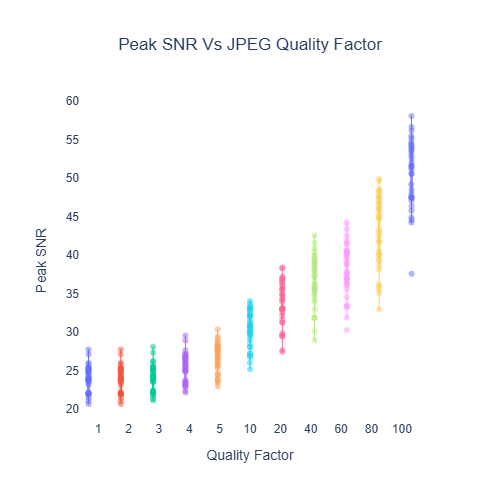
\includegraphics[width=0.5\textwidth]{assets/JPEG Quality Factor and PSNR.png}
    \caption{Quality factor vs PSNR}
    \label{fig:psnr_jpeg}
\end{figure}

\begin{figure}
    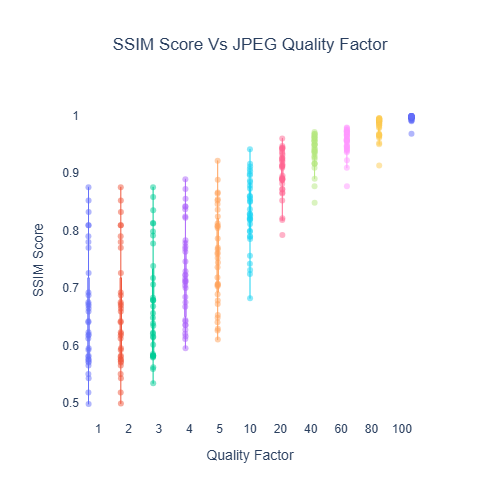
\includegraphics[width=0.5\textwidth]{assets/JPEG Quality factor and SSIM Score.png}
    \caption{Quality Factor vs SSIM}
    \label{fig:ssim_jpeg}
\end{figure}

\begin{figure}
    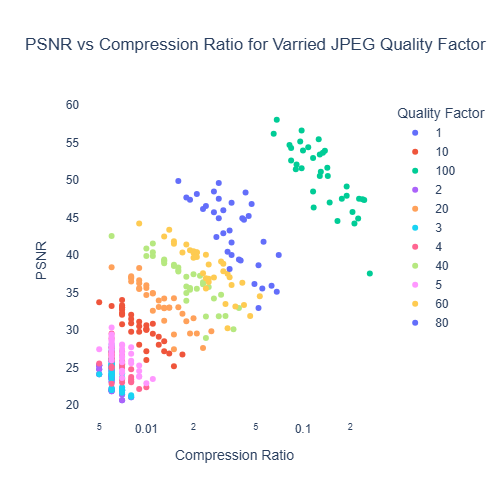
\includegraphics[width=0.5\textwidth]{assets/JPEG Compression Ratio Vs PSNR.png}
    \caption{PSNR Vs Compression Rate for a variety of Quality Factors}
    \label{fig:psnr_vs_compression_ratio}
\end{figure}

\subsubsection{Compression Quality Vs Quantization}

Using our flexible compression framework, quantization is varied according to table \ref{tab:Quantization-Parameters-Table} and \ref{tab:Quantization-Parameters-LN-Norm}. These quantizations are applied to images with an additional 2x chrominance downsampling applied to them.

Interestingly, when compraing compression ratio to PSRN, there is a clear bifurcation as the quantization rate increases. Some images experience a clear increase in PSNR as the compression rate is increased, consistent with the results from the JPEG baseline. However, many of the images see hardly any increase in PSRN as the compression ratio increases \ref{fig:gauss_quantization_vs_psnr}. Taking a closer look at these images, it appears that the images for which PSRN does not correlate to compression ratio are the high or very high quality images in the dataset, with dimensions on the order of \~ 6000 x 4500. Since for all quantizations, there is a chrominance downsample factor applied, for these large images, this is likley the cause of the degrated PSNR. For images with smaller starting dimensions, a 2x chromiance downsample factor does not remove as much information, so it's expected that the PSNR would not be as degraded.

\begin{figure}
    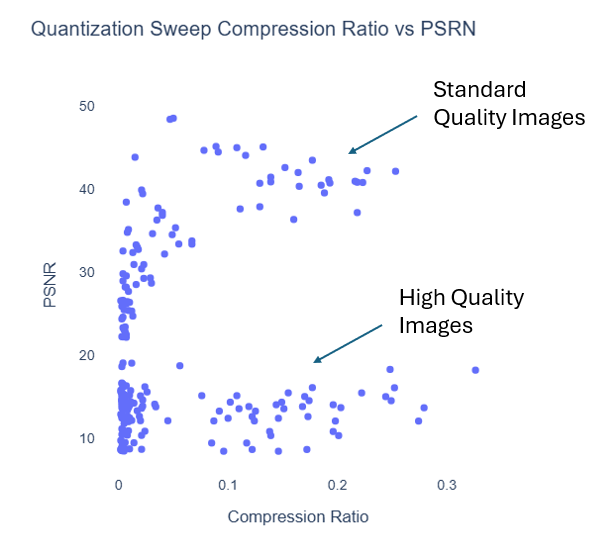
\includegraphics[width=0.5\textwidth]{assets/Quantization Sweep Compression Ratio vs PSRN.png}
    \caption{PSRN vs Compression Ratio across a sweep of quantizations defined in table \ref{tab:Quantization-Parameters-Table}. Clear bifurcation shows that images with larger starting dimensions suffer more from even a modest 2x chrominance downsample factor}
    \label{fig:gauss_quantization_vs_psnr}
\end{figure}

\subsubsection{LN-Norm Quantization}

Along with having the ability to fine-tune the exact quantization parameters, our flexible compression pipeline also gives the ability to generate quantization matricies with different structures. Here we evaluate if the relative quantization of mid-range frequences relative to high and low frequencies can help improve performance without resulting in additional file size. Unfortunately, there is little to no change in the relationship between PSNR and compression rate as the norm N is varied, or even comprared to the Gaussian Weight quantization, as shown in figure \ref{fig:LN-norm_quantization_performance}

\begin{figure}
    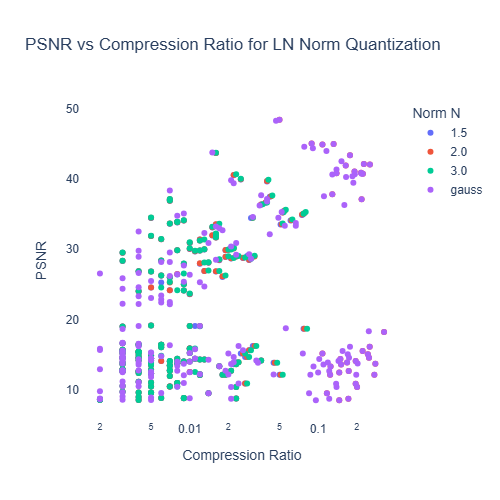
\includegraphics[width=0.5\textwidth]{assets/PSNR for LN Quantization with gaussian weights.png}
    \caption{PSRN vs compression ratio for a variety of quantization weights. Changing the relative rates of quantization for mid-range frequencies has no impact on the relationship between the image PSNR and the compression rate.}
    \label{fig:LN-norm_quantization_performance}
\end{figure}

In addition to there being very little change in the compression ratio, LN-normalized images look visible more degraded, as shown in figure \ref{fig:quantization_function_comparison}

\begin{figure}
    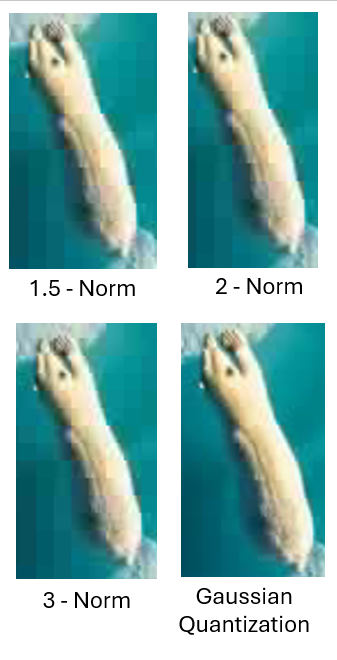
\includegraphics{assets/Quantization Function Comparison.png}
    \caption{LN-norm quantization results compared to Gaussian Quantization weights}
    \label{fig:quantization_function_comparison}
\end{figure}

\subsubsection{Chrominance Downsampling}

JPEG leverages a YCbCr colorspace in order to distinguish between Luminance and Chrominance information in the image.
This distinction allows for the Chrominance Channels to be downsampled while the Luminance stays full rank.
In this section we analyze the effects of downsampling on our compressed image quality metrics. 
Shown in figure \ref{fig:downsample_vs_psnr}, downsampling uniformly reduces PSNR and compression rate. However, unlike Quantization, image quality drops off steeply and compression rate does not improve significatly for large downsample factors.

\begin{figure}
    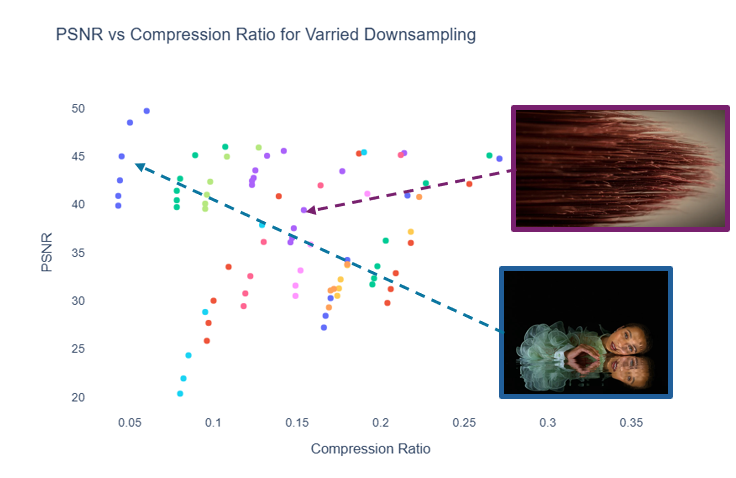
\includegraphics[width=0.5\textwidth]{assets/PSNR vs Chromiance Downsampling with Images.png}
    \caption{As expected, generally increasing the chromiance downsample rate (and therefore reducing the compression ratio), the PSRN metric is degraded.}
    \label{fig:downsample_vs_psnr}
\end{figure}

\subsubsection{Block Size}

For this experiment we vary the block size according to table \ref{tab:Block Size Sweep}. We find the larger blocks do not compress the images as much as small blocks \ref{fig:block_comp_rates}. Additionally, varrying the block size also does not see to effect the PSNR to a large extent. However, qualitatively the blocking strategies are visibly different \ref{fig:block_quantization_artifacts}. The effect of smaller blocks is that the edges of each block becomes more clearly visible, giving the effect that the entire image has been downsampled in 2x2 pixel blocks. In larger blocks, there are shimmers and other quantization artifacts which are visible across the block upon close inspection, despite the block edges being less obvious. It's clear that a small block with a reasonable compression rate, that preserves a gradient over the block while minimizing frequency quantization artifacts is ideal for image visual appeal.

\begin{figure}
    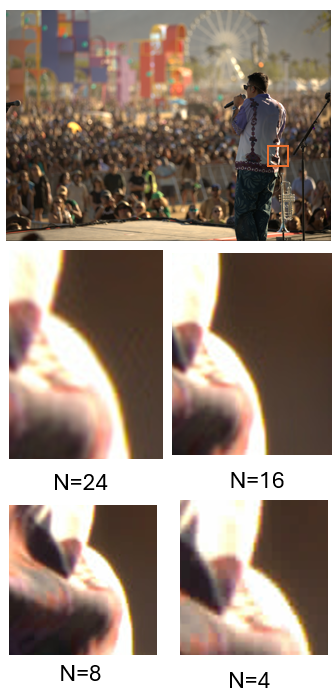
\includegraphics[width=0.5\textwidth]{assets/Block Quantization Artifacts.png}
    \caption{A visualization of block size artifacts. As blocks become larger, individual blocks have more detail, and features within the blocks are more clear, but block boundaries are still visible.}
    \label{fig:block_quantization_artifacts}
\end{figure}

\begin{figure}
    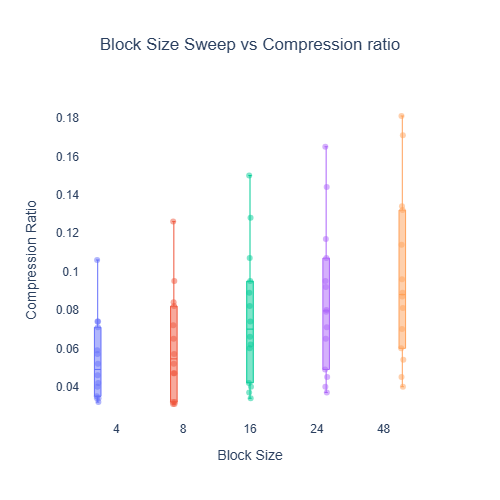
\includegraphics[width=0.5\textwidth]{assets/Comp Rate VS block Size.png}
    \caption{Compression Rates improve with smaller block sizes, while larger block sizes result in overall larger image size, despite the same relative quantization being applied across block sizes.}
    \label{fig:block_comp_rates}
\end{figure}

\begin{figure}
    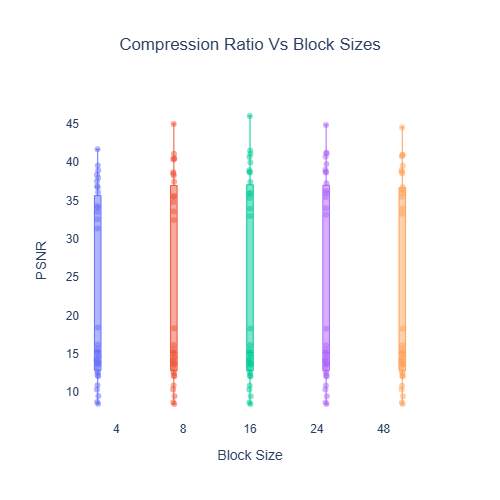
\includegraphics[width=0.5\textwidth]{assets/Block Size Vs PSNR.png}
    \caption{As block size is varried with quantization kept relativly the same, the PSNR does not change.}
\end{figure}

\subsubsection{Compression Quality Discussion}

By far the most effective way to reduce image file size while maintaining high image quality metrics is to apply a moderately agressive quantization on relativly small blocks. In order for this quantization to be successful, high frequencies need to be heavily attenuated while low frequencies are maintained. Other modifications or factors swept either resulted in a very fast degradation of image quality with little change in compression ratio, or did not siginificantly effect either metric while introducing undesireable visual artifacts.

\subsection{Semantic Preservation}
Images were evaluated using a pre-trained classification model (e.g., ResNet50) to test whether compression degrades semantic content. This was done using \texttt{test/classification\_tests.py}.

\textbf{TODO: Replace charts in this section with ones that have clearer labels and axis titles.}

\subsubsection{Test Images for Semantic Preservation}

In order to evaluate our compression pipeline, a set of test images with a variety of objects for classification was chosen. 
Resnet50 is a model largely for objects and non-human subjects, so images with a clear subject well centered in the image, spanning range of sizes relative to the size of the image. 
Additionally, some images were deliberately chosen because they contain multiple subjects or subjects where the classification is somewhat ambiguous, to see if these are more adversely effected by the compression than clear images, see figure \ref{fig:test_images} for the continum of subjects tested. 
All test images are evaluated against all compression configurations. A set of novel images for classification are chosen for benchmarking rather than ImageNet or ResNet training set images to avoid compounding effects of muliple lossy compressions on the image. 
ImageNet and ResNet images are already JPEG images, and therefore have some (unknown) level of compression already applied to them. The test set images are either raw formats or lossless image formats (such as .png, and .webp).

\begin{figure}
    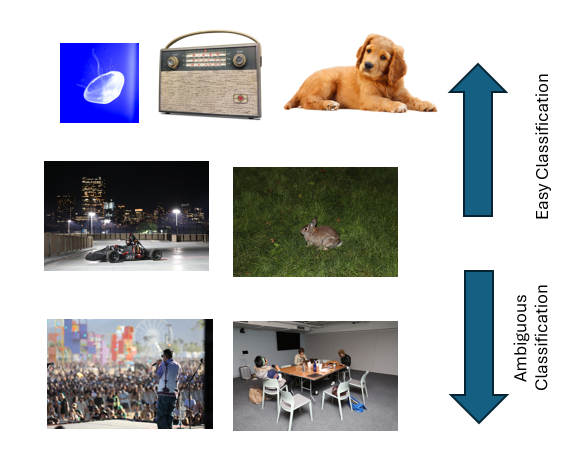
\includegraphics{assets/Classification Sweep.png}
    \caption{Images are chosen for classification with a variety of subjects and easy of classification.}
    \label{fig:test_images}
\end{figure}

\subsubsection{JPEG Compression as a baseline for Semantic Preservation}

As a natural starting point of comparison for Semantic Preservation, we evaluate the semantic preservation of the JPEG compression standard.
The JPEG standard only exposes a single compression parameter available for adjustment, the JPEG Quality Factor (QF) largly effects the quantization table values for each of the Descrete-Cosine-Transformed Blocks.
Images are evaluated for semantic preservation using algorithm \ref{fig:Annotated JPEG Baseline}.
Results are then parameterized by compression rate and original image content (figure \ref{fig:Comp vs Ratio JPEG Baseline}). There appears to be an inflection point around compression ratios of 0.1 or less, where certain images loose nearly all of their semantic content. For certain images, even ratios of 0.01 do not increase confidence error.

Taking a closer look at these images, images where the subject is large relative to the frame of the image have their semantic classifications more well preserved even with extremely agressive compression. However, When images contain other objects than the subject, or the subject of the image is small, the compression has a more dramatic impact on the classification. This trend is highlighted in figure \ref{fig:Annotated JPEG Baseline}

\begin{figure}
    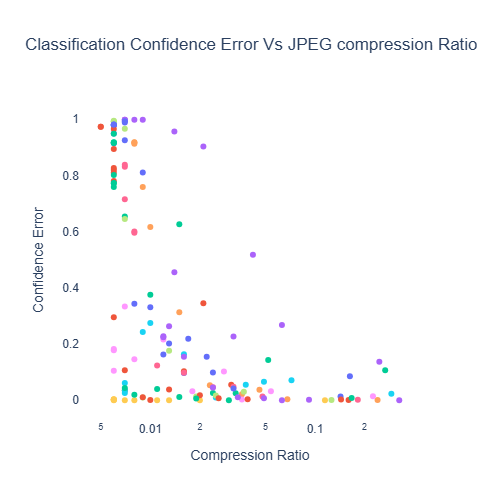
\includegraphics[width=0.5\textwidth]{assets/Baseline JPEG Confidence vs Comp Ratio.png}
    \caption{Confidence Error vs Compression Ratio for JPEG Compression. Smaller Values on the X axis correspond to smaller compressed images, while higher values on the Y axis correspond to a higher classification error rate. It appears that compression rates have little to no effect on semantic content until the compression ratio dips below 0.1.}
    \label{fig:Comp vs Ratio JPEG Baseline}
\end{figure}

\begin{figure}
    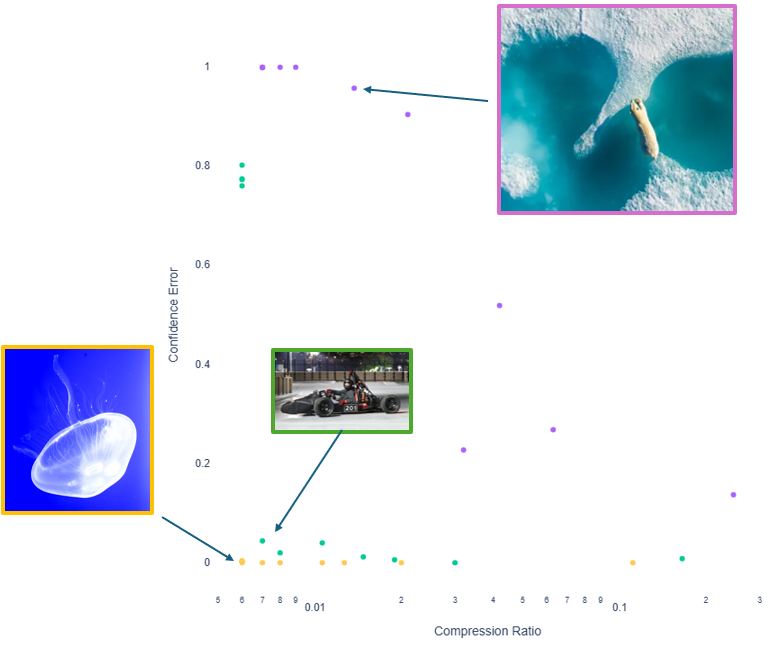
\includegraphics[width=0.5\textwidth]{assets/JPEG Baseline Compression with Examples}
    \caption{Certain Images have their semantic content preserved even with extremely agressive compression parameters where images are reduced to 0.6\% of their original size. Other images suffer from a sharp decline preserved semantic information. Intuitively, the higher the percentage of pixels in the image that represent the subject of classificatoin (as in the case of the jellyfish and the racecar), the better semantic preservation through compression.}
    \label{fig:Annotated JPEG Baseline}
\end{figure}

The results for JPEG compression on these test images can serve as a baseline for other compression parameters evaluated.

\subsubsection{Quantization Sweep Results}

One of the compression parameters that our flexible compression pipeline makes available are the Quantization Tables.
These can be generated using Gaussian of the bottom right distance or scaled min and max values by the L-N Norm distances.
When Quantization is increased, more of the high-frequency information of the image is lost, so by sweeping through a set of quantization parameters, we can demonstrate the relative sensitivity of semantic information on high vs low frequency components.
The flexible compression pipeline also enables setting of luminance and chrominance quantization seperately, so we can explore whether semantic information is more closely tied to Luminance, or Chrominance information.

The parameters for Chrominance and Luminance quantization tested are listed in table \ref{tab:Quantization-Parameters-Table}. For sweeps with just Luminance or just Chrominance varied, the other quantization channel is processed with no Quantization.
All experiments use a Chrominance downsample factor of 2.

Similar to the JPEG baseline, Confidence Error increases sharply when the compression rate drops below 0.1, as shown in figure \ref{fig:Confidence vs Quantization}
Interestingly however, when just the Chrominance or just the Luminance channels are varied, both the Confidence error and the compression ratio suffer. Shown in figure \ref{fig:just chroma or luma downsampling}
\begin{figure}
    \label{fig:Confidence vs Quantization}
    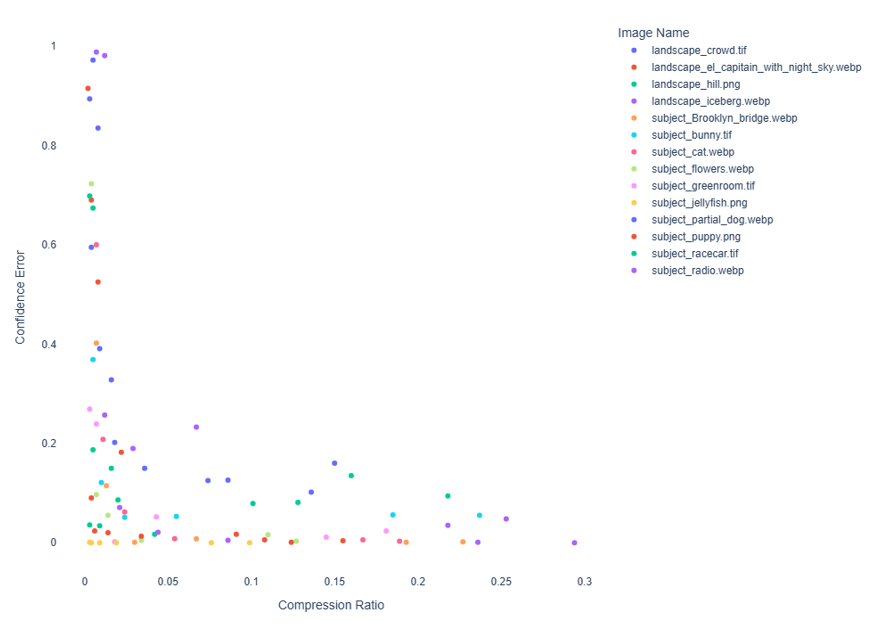
\includegraphics[width=0.5\textwidth]{assets/Quantization Sweep No Title Chrominance and Luminance.png}
    \caption{Confidence Error vs Compression Ratio as the Quantization parameters are varied. Quantization has very little effect on Semantic information until the compression ratio gets below approximately 0.1.}
    \label{fig:Confidence vs Quantization}
\end{figure}
\begin{figure}
    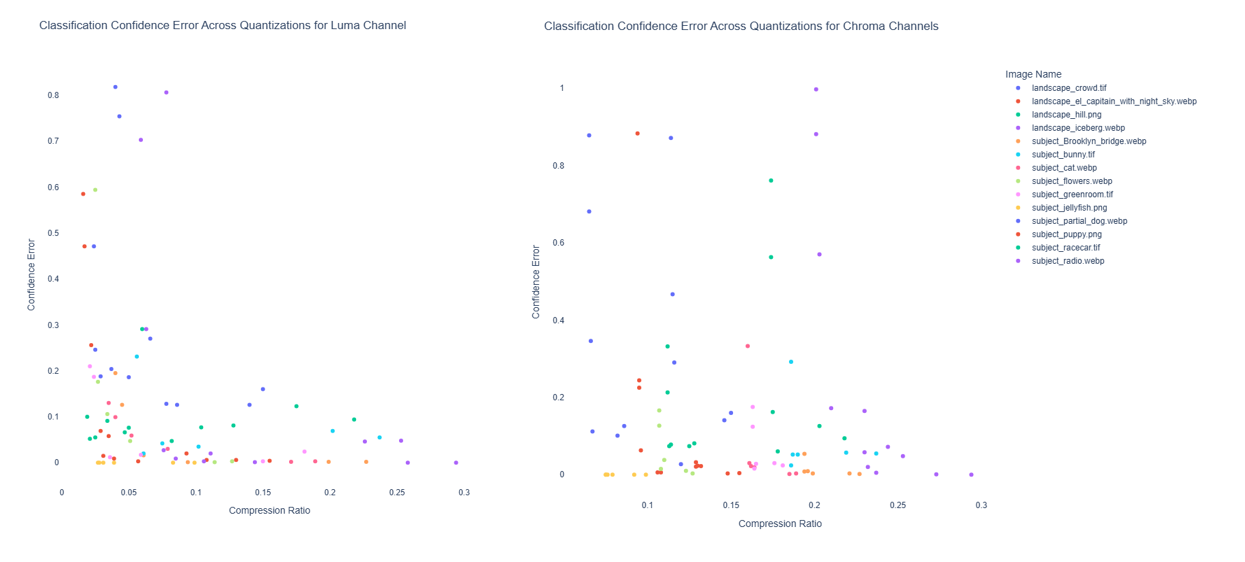
\includegraphics[width=0.5\textwidth]{assets/Chroma and Luma downsampling combined.png}
    \caption{Unlike in \ref{fig:Confidence vs Quantization}, if just one of the channel types is quantized, the semantic information is quickly lost, and the compression ratio is not improved.}
    \label{fig:just chroma or luma downsampling}
\end{figure}

\subsubsection{Block Size}

Block size affects the compressed result by changing pixel block base unit the Descrete Cosine Transform operates on.
Larger Blocks include a wider range of frequencies and more information being transformed each time, while smaller blocks allow for discontinuities at block edges to potentially go unnoticed.
In this experiment, we test apply our compression to images while varrying block size.

\begin{figure}
    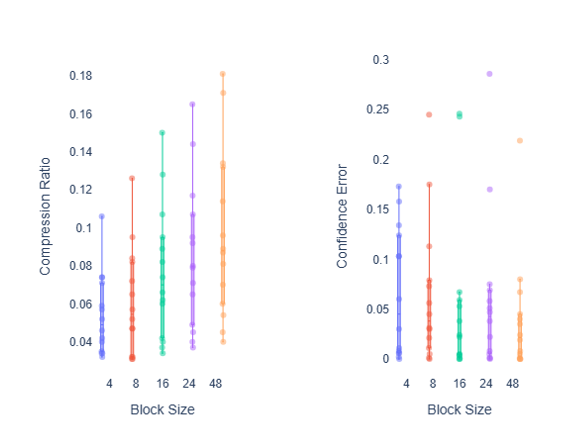
\includegraphics[width=0.5\textwidth]{assets/Confidence Err Vs Block Size.png}
    \caption{Confidence Error vs Compression Ratio for a variety of block sizes. As with other swept parameters, compression ratio and confidence error are inversely related.}
    \label{fig:block_size_sweep}
\end{figure}

\subsubsection{Discussion}

Similar to compression quality, among all tested parameters, quantization proved the most effective in reducing image file size while preserving semantic information. However, some other interesting trends arrise. If quantization is applied to only one of the channels, even if that is the chromiance chaannel only, the Confidence Error increases significantly over relativly modest Compression Ratios. This suggests that there is Semantic meaning encoded in color information in a different color space the YCbCr color. Future work could include applying different color transformations to the image before quantizing.

\subsection{Runtime and Performance}
Execution time for both compression and decompression is measured and stored during sweeps. Aggregate runtime plots can be shown here.

One main difference between our compression pipeline and JPEG compression is that the huffman tables are not pre-computed. Through our tests we note that this accounts for a significant portion of the computational load for compression and decompression \ref{fig:runtimes}. It is important to note that these runtimes are not comparable to well established codex standards, as most machines have dedicated hardware for performing these computations. The computed runtimes are only comparable to other internal results. 

\begin{figure}
    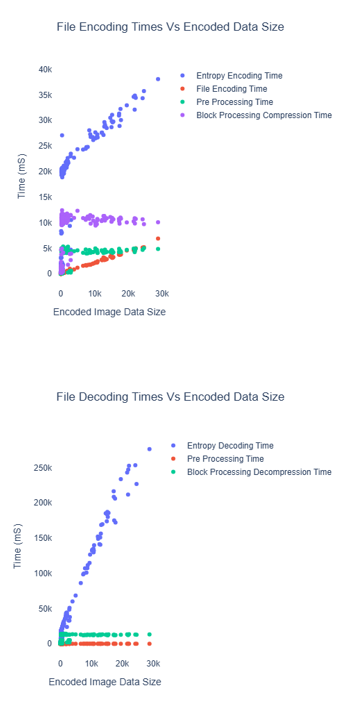
\includegraphics[width=0.5\textwidth]{assets/Runtimes Summary.png}
    \caption{Sets of sampled runtimes for the most computationally intensive parts of the our flexible compressoin pipeline.}
    \label{fig:runtimes}
\end{figure}

